% +----------------------------------------------------------------------------+
% | Instituto Nacional de Pesquisas Espaciais - INPE
% | ----------------------------------------------------------------------------
% | Authors     : M. E. G. Borges; M. L. S. Nascimento; J. E. C. Cruz
% | Version     :
% | Copyright   :
% | Description : Registro e Mosaico de Imagens Obtidas por VANTs
% +----------------------------------------------------------------------------+

\documentclass[9pt, a4paper, nofonttune, journal]{IEEEtran}
\usepackage[utf8x]{inputenc}
\usepackage[T1]{fontenc} % permite copiar texto com acento em PDF
\usepackage{url}
\usepackage{graphicx}
\usepackage{amsmath}%pacote necessário para a utilização de algumas funções matemáticas nas formulas
\usepackage{float}%responsável por o posicionamento de figuras

% correct bad hyphenation here
\hyphenation{di-fe-ren-tes trans-for-ma-coes es-pe-ci-al-men-te}


\begin{document}

\title{Registro e Mosaico de Imagens \\Obtidas por Câmera Digital a bordo de VANT}

\author{
  \IEEEauthorblockN{
    Marcos Eduardo Gomes Borges \IEEEauthorrefmark{1}\\
    Marina Laís da Silva Nascimento \IEEEauthorrefmark{1}\\
    Juliano E. C. Cruz \IEEEauthorrefmark{1}\\
    Leila Maria Garcia Fonseca \IEEEauthorrefmark{2} \linebreak\linebreak
  }
  \IEEEauthorblockA{
    Instituto Nacional de Pesquisas Espaciais – INPE\\
    Programa de Mestrado em Computação e Matemática Aplicada \IEEEauthorrefmark{1}\\
    Divisão de Processamento de Imagens \IEEEauthorrefmark{2}\\
    São José dos Campos, Brasil\\
    \{marcoseborges, marina.lsnascimento, juliano.ecc\}@gmail.com, leila@dpi.inpe.br
  }
}

% The paper headers
\markboth{Journal of DPI-INPE,~Vol.~XX, No.~1, Janeiro~2012}%
{Shell \MakeLowercase{\textit{et al.}}: Trabalho de PDI - INPE}

\maketitle               
\renewcommand\abstractname{Resumo}
\renewcommand{\refname}{Referências}
\renewcommand\IEEEkeywordsname{Palavras-chave}


\begin{abstract}
Neste trabalho comparamos dois algoritmos de registro de imagens implementados na biblioteca TerraLib: Optical Flow e Operador Moravec Modificado. Através da comparação desses algoritmos implementamos uma solução híbrida para registrar e mosaicar imagens adquiridas por câmera digital a bordo de VANT.
\end{abstract}

\begin{IEEEkeywords}
Registro de Imagens, Mosaico, VANT, TerraLib.
\end{IEEEkeywords}

\section{Introdução}
A utilização de Veículos Aéreos não Tripulados (VANTs) tem apresentado grande crescimento nos últimos anos devido a diversos fatores, tais como ausência de tripulação em tarefas tediosas, cansativas ou que envolvem riscos à tripulação, baixo custo operacional e de fabricação comparados às aeronaves convencionais, entre outros. Imagens aéreas obtidas através de VANTs possuem grandes aplicações \cite{Canhoto} e o objetivo geral deste trabalho é realizar registro e mosaico de imagens adquiridas por aeronaves não tripuladas. O mosaico de sequências de imagens aéreas apresenta alguns problemas de distorções geométricas devido às variações de altitudes da aeronave e distorções devido as diferenças de escala, projeção e ângulo de visada em cenas de baixa altitude e que apresentam prédios e montanhas. Outro problema também enfrentado ao gerar o mosaico nesse tipo de imagem, é que quando a aeronave realiza curvas para seguir o plano de voo traçado captura imagens com sistema de coordenadas rotacionadas em ângulos diferentes e desconhecidos, e isso também gera distorções que buscamos resolver neste trabalho.

Na Figura~\ref{fig:plano_voo} pode-se observar o exemplo de um plano de voo para um VANT. Neste trabalho, as imagens adquiridas pela câmera digital a bordo da aeronave não possuem georeferenciamento e são coletadas a cada um segundo. Após o término da aquisição das imagens, as mesmas necessitam ser mosaicadas. O procedimento inicial para essa tarefa é o registro de imagens, que inicia a busca por correspondências entre imagens diferentes que representam a mesma cena \cite{Fonseca:1999:ReAuIm}. Neste trabalho, a busca por correspondências entre pontos de imagens diferentes é realizada e comparada entre dois algoritmos: Optical Flow e Operador Moravec Modificado, ambos implementados na biblioteca TerraLib.

\begin{figure}[H]
\begin{center}
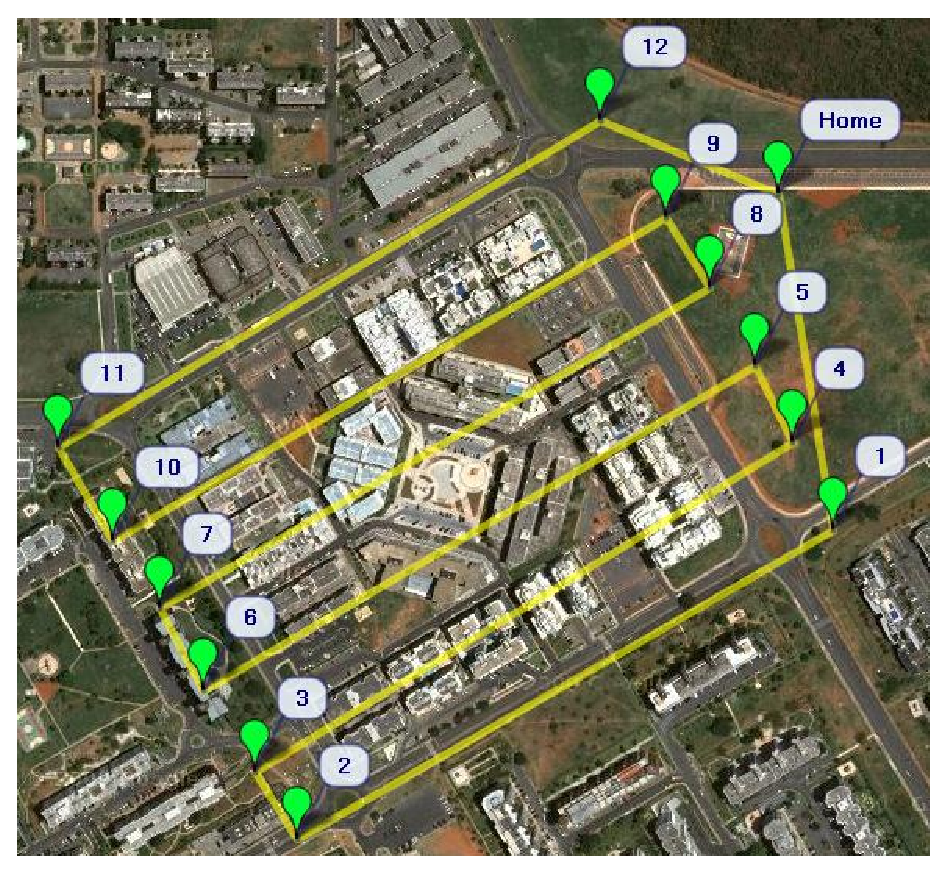
\includegraphics[scale=0.50]{figuras/plano_voo}
\caption{Exemplo de Plano de Voo do VANT}
\label{fig:plano_voo}
\end{center}
\end{figure}

\section{Registro e Mosaico de Imagens}
O registro de imagens pode ser entendido como um processo de casamento entre duas imagens que possuem uma área comum.
A imagem tomada como base de registro é chamada de imagem de referência e a imagem a ser registrada é chamada de imagem de ajuste.
O processo basicamente envolve três etapas:
\begin{enumerate}
	\item Obtenção de pontos de controle;
	\begin{enumerate}
		\item Extração de feições;
		\item Casamento das feições extraídas;
	\end{enumerate}
	\item Determinação da função de transformação;
	\item Sobreposição das imagens.
\end{enumerate}

As imagens a serem registradas podem ser relacionadas através de função de transformação simples se a geometria das imagens for semelhante.
Se a geometria das imagens for diferente, as transformações podem ser aproximadas utilizando um função polinomial cujos parâmetros são determinados 
a partir das coordenadas dos pontos de controle.
O número de pontos de controle representa a situação de um sistema de equações determinado.
Entretanto, como as coordenadas medidas dos pontos de controle estão sujeitas a erros, convém usar um número de pontos maior que o número mínimo,
o que define um sistema de equações sobredeterminado.

O produto gerado através das técnicas de registro de imagens é o mosaico, que nada mais é do que uma 
composição de imagens adquiridas de diferentes pontos de vista visando construir uma imagem maior, permitindo assim uma visão global da cena.\cite{Fedorov1}

Neste trabalho a biblioteca utilizada para a realização do registro e mosaico foi a TerraLib, que é uma biblioteca \textit{open source} de classes e funções SIG disponível na Internet, possibilitando portanto, um ambiente colaborativo e seu uso para o desenvolvimento de novas ferramentas. Atualmente é desenvolvida pelo INPE, PUC-Rio e FUNCATE \cite{Terralib1}. A utilização desta biblioteca se deu em todas as etapas necessárias para a realização do registro e mosaico das imagens, ou seja, na obtenção de pontos de controle, na transformação espacial da imagem e na sobreposição das imagens.

\subsection{Detecção de pontos de controle}
Ponto de interesse é como é chamado qualquer ponto de uma imagem em que o sinal tenha uma mudança bidimensional. Cantos ou ângulos no formato L, T e Y obecem essa definição assim como pontos pretos em um fundo branco, o final de ramificações ou qualquer textura bidimensional significante \cite{Coderlia1}. Ponto de controle são, portanto, os pontos de interesse em imagens de sensoriamento remoto que são utilizados para aplicar transformações geométricas afim de realizar o processo de registro entre as determinadas imagens.\cite{Schowengerdt}

\subsubsection{Detector Moravec}
O detector Moravec foi uma dos primeiros detectores de ponto de interesse a serem desenvolvidos, sendo descrito primeiramente 
em 1977 por Hans Moravec \cite{Moravec1}. Esse detector é baseado na função de auto-correlação do signal. Ele compara as diferenças de nível de cinza entre a janela atual e de janelas 
deslocadas em quatro direções paralelas à colunas e linhas. Se o mínimo dessas quatro diferenças é superior a um determinado limiar, então um ponto de interesse
foi encontrado \cite{Coderlia1}.
  
O operador Moravec pode ser definido matematicamente como:
    \begin{center}$V_{1}=\frac{1}{p(q-1)}\sum_{i=-k}^k\sum_{j=-l}^{l-1}\bigl(g(i,j)-g(i,j+1)\bigr)^2$    \end{center}
    \begin{center}$V_{2}=\frac{1}{(p-1)q}\sum_{i=-k}^{k-1}\sum_{j=-l}^l\bigl(g(i,j)-g(i+1,j)\bigr)^2$    \end{center}
    \begin{center}$V_{3}=\frac{1}{(p-1)(q-1)}\sum_{i=-k}^{k-1}\sum_{j=-l}^{l-1}\bigl(g(i,j)-g(i+1,j+1)\bigr)^2$\end{center}
    \begin{center}$V_{4}=\frac{1}{(p-1)(q-1)}\sum_{i=-k}^{k-1}\sum_{j=-l}^{l-1}\bigl(g(i,j+1)-g(i+1,j)\bigr)^2$\end{center}
    \begin{center}$V = min(V1,V2,V3,V4)$\end{center}

    Onde $p = 2k + 1$ e $q = 2l + 1$, sendo que $k\times l$ o tamanho da janela utilizada.

Na biblioteca TerraLib, o método Moravec é implementado pela classe \texttt{TePDIMMIOMatching}.

\subsubsection{Optical Flow}
Fluxo ótico é a distribuição de velocidades aparentes do movimento de padrões de brilho em uma imagem \cite{GibsonBook1}. Assim, pode-se obter informações importantes a respeito da distribuição espacial dos objetos visualizados e da taxa de mudança dessa distribuição. Discontinuidades do fluxo ótico podem ajudar a segmentar uma determinada imagem em regiões que correspondem a diferentes objetos. Esse conceito começou a ser estudado na década de 1940 e foi publicado primeiramente pelo psicólogo James Gibson \cite{Gibson1} \cite{OF1}.

Um pixel tendo a localização $(x,y,t)$ com intensidade $I$ será movido em $\Delta x$, $\Delta y$ e $\Delta t$ entre os quadros de uma mesma imagem. Assim, chega-se a equação:

\begin{center}
$\frac{\partial I}{\partial x}\frac{\Delta x}{\Delta t}+\frac{\partial I}{\partial y}\frac{\Delta y}{\Delta t}+\frac{\partial I}{\partial t}\frac{\Delta t}{\Delta t} = 0 $\end{center}

simplificando tem-se que,

\begin{center}
$\frac{\partial I}{\partial x}V_x+\frac{\partial I}{\partial y}V_y+\frac{\partial I}{\partial t} = 0$\end{center}

Onde $V_x$ e $V_y$ são os componentes $x$ e $y$ do fluxo ótico.

Na biblioteca TerraLib, o método Optical Flow ou é implementado pela classe \texttt{TePDIOFMatching}.

\subsection{Casamento de pontos de controle}
Após se obter os pontos de controle de ambas as imagens em que deseja-se realizar o registro, é necessário descobrir qual é o ponto da imagem de ajuste correspondente à um determinado ponto na imagem de referência.

\subsubsection{Correlação cruzada normalizada}
O funcionamento do método estatístico de correlação cruzada normalizada se dá ao extrair pequenas janelas ao redor de cada ponto de controle nas duas imagens. Aplica-se então, aos pares o método(descrito abaixo) entre todas as janelas obtidas na imagem de referência com as obtidas na imagem de ajuste \cite{Fedorov1}\cite{Leila1}\cite{Zhao1}.

\begin{center}
$R(i,j)=\frac{\overset{K-1}{\underset{l=0}{\sum}}\underset{m=0}{\overset{L-1}{\sum}}W_{z}(l,m)\cdot S_{ij}(l,m)}{\sqrt{\overset{K-1}{\underset{l=0}{\sum}}\underset{m=0}{\overset{L-1}{\sum}}W_{z}^{2}(l,m)\overset{K-1}{\underset{l=0}{\sum}}\underset{m=0}{\overset{L-1}{\sum}}S_{ij}^{2}(l,m)}}$\end{center}
Onde $S_{ij}$ é a janela da imagem de referência e $W_{z}$ a janela da imagem de ajuste.
Assim, quanto maior valor de $R(i,j)$ maior é a semelhança entre as duas janelas comparadas.
O TerraLib implenta esse método de casamento em suas classes.

\subsection{Transformações Geométricas}
Com o casamento dos pontos de controle já realizado, agora é necessário aplicar funções de transformação geométrica para que se possa ter a imagem de ajuste adequada geometricamente e espacialmente afim de sobrepor as imagens obtendo o mosaico.

Transformação geométrica é o nome que se dá à aplicação de uma determinada função matemática em uma determinada figura geométrica em que o resultado é geometricamente igual ou semelhante à figura original. Abaixo temos as transformações elementares:

\subsubsection{Translação}
A translação desloca um determinado ponto ou conjunto de pontos uma determinada distância em um determinado sentido.

\begin{center}
$\begin{bmatrix}x'\\
y'
\end{bmatrix}=\begin{bmatrix}x\\
y
\end{bmatrix}+\begin{bmatrix}t_{x}\\
t_{y}
\end{bmatrix}$\end{center}
Onde $t_{x}~~ \textrm{e} ~~ t_{y}$ são respectivamente as taxas de translação no eixo $x~~ \textrm{e} ~~y$~\cite{CGPPBook1}.

\begin{figure}[H]
\begin{center}
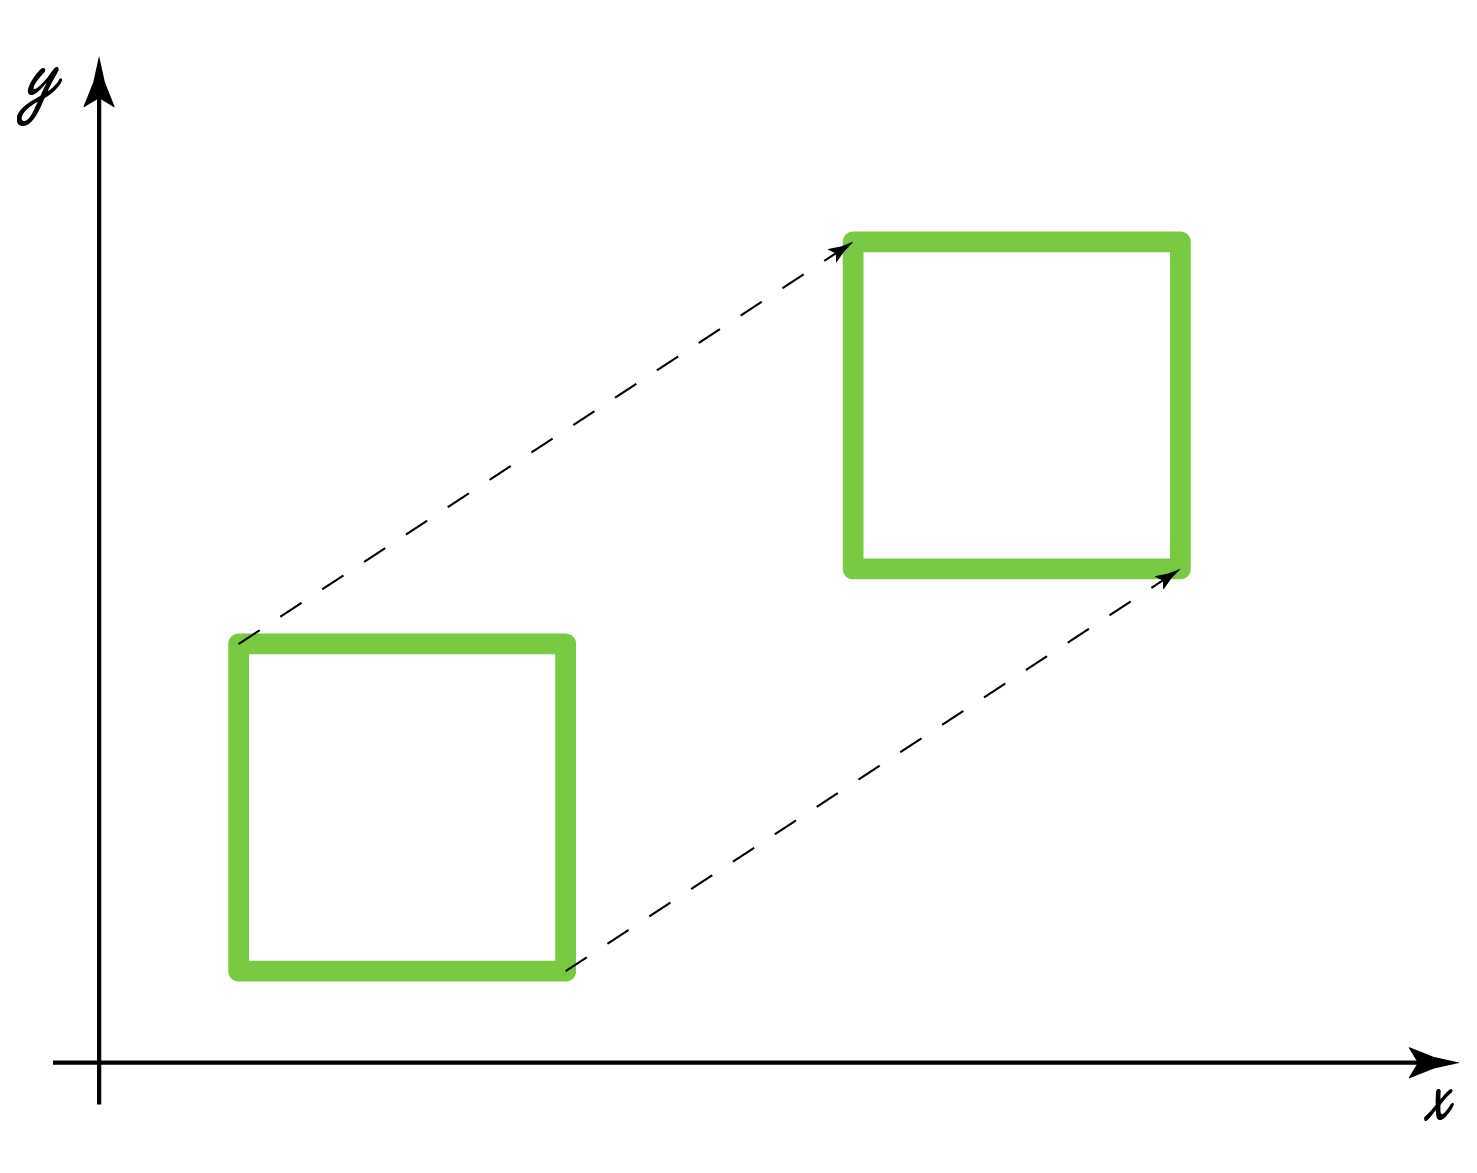
\includegraphics[scale=0.25]{figuras/translation1}
\caption{Exemplo de translação em um espaço bidimensional}
\end{center}
\end{figure}

\subsubsection{Variação de escala}

A variação de escala é o fato de se esticar ou encolher uma determinada figura em relação ao eixos $x$ e $y$.

\begin{center}
$\begin{bmatrix}x'\\
y'
\end{bmatrix}=\begin{bmatrix}v_{x} & 0\\
0 & v_{y}
\end{bmatrix}\begin{bmatrix}x\\
\frac{}{}y
\end{bmatrix}$\end{center}
Onde $v_{x}~~ \textrm{e} ~~ v_{y}$ são respectivamente as taxas de escala no eixo $x~~ \textrm{e} ~~y$~\cite{CGPPBook1}.

\begin{figure}[H]
\begin{center}
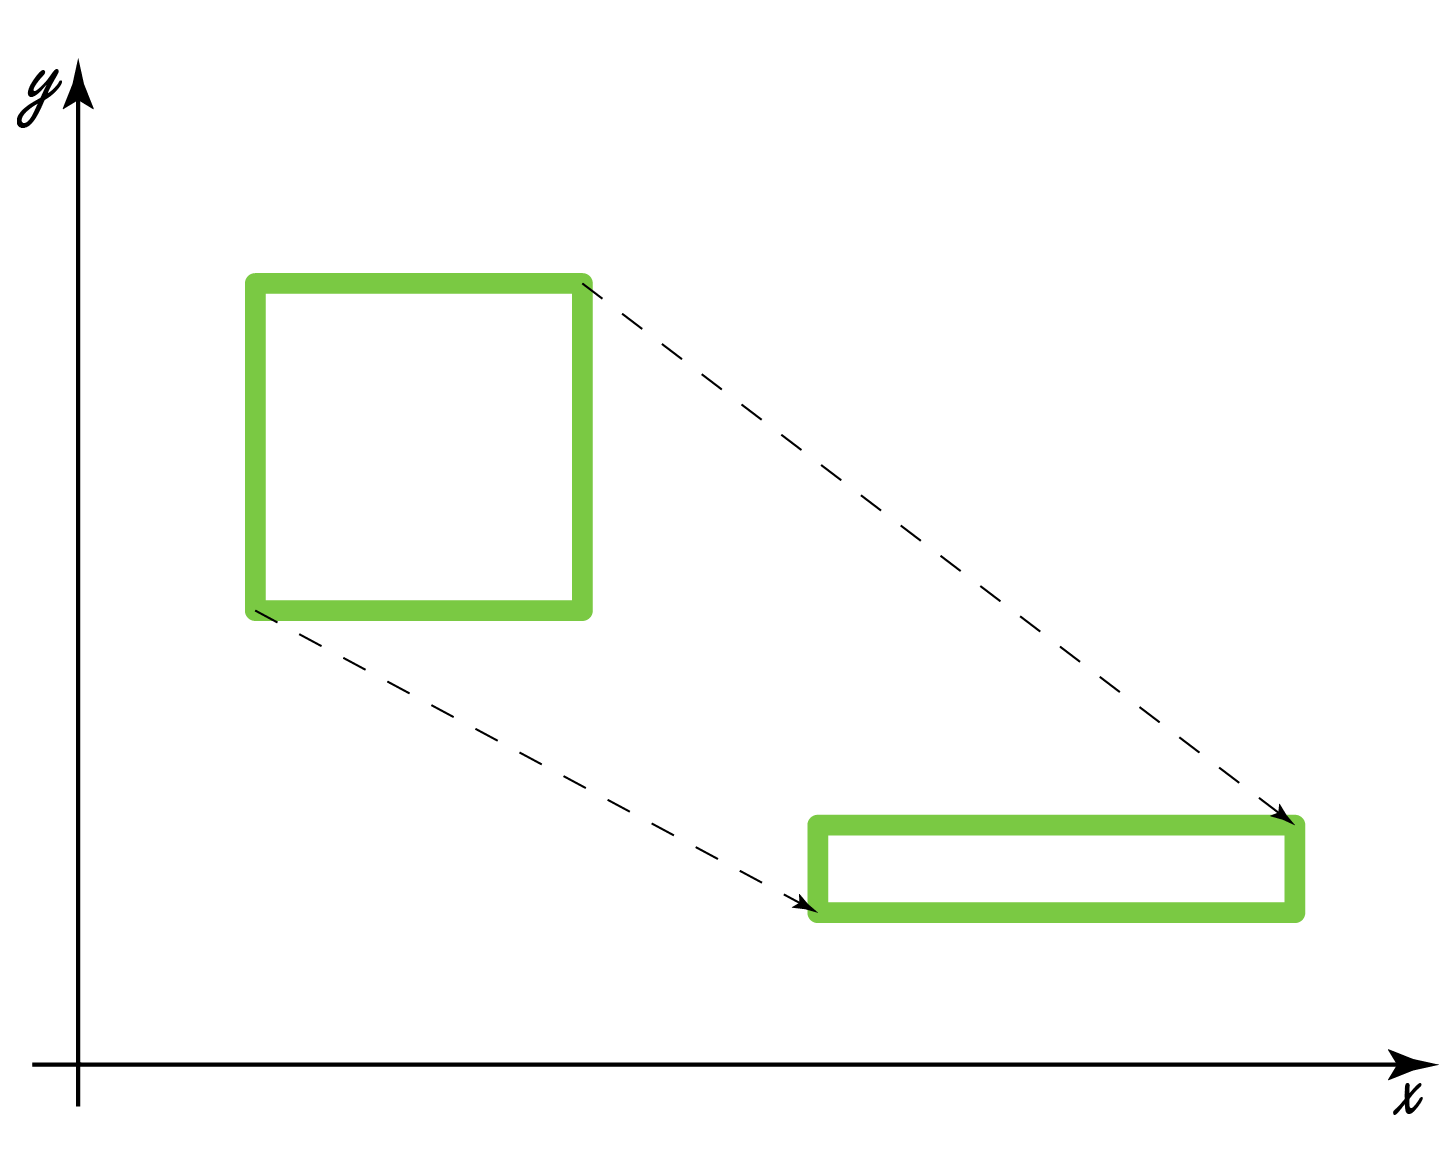
\includegraphics[scale=0.25]{figuras/scale1}
\caption{Exemplo de variação de escala em um espaço bidimensional}
\end{center}
\end{figure}

\subsubsection{Rotação}
Na rotação rotaciona-se a figura em torno de um determinado eixo.

\begin{center}
$\begin{bmatrix}x'\\
y'
\end{bmatrix}=\begin{bmatrix}cos\theta & -sen\theta\\
cos\theta & sen\theta
\end{bmatrix}\begin{bmatrix}x\\
y
\end{bmatrix}$\end{center}
Onde $\theta$ é o ângulo que a figura será rotacionada em relação a posição original levando em consideração a origem como eixo \cite{CGPPBook1}.

\begin{figure}[H] 
\begin{center}
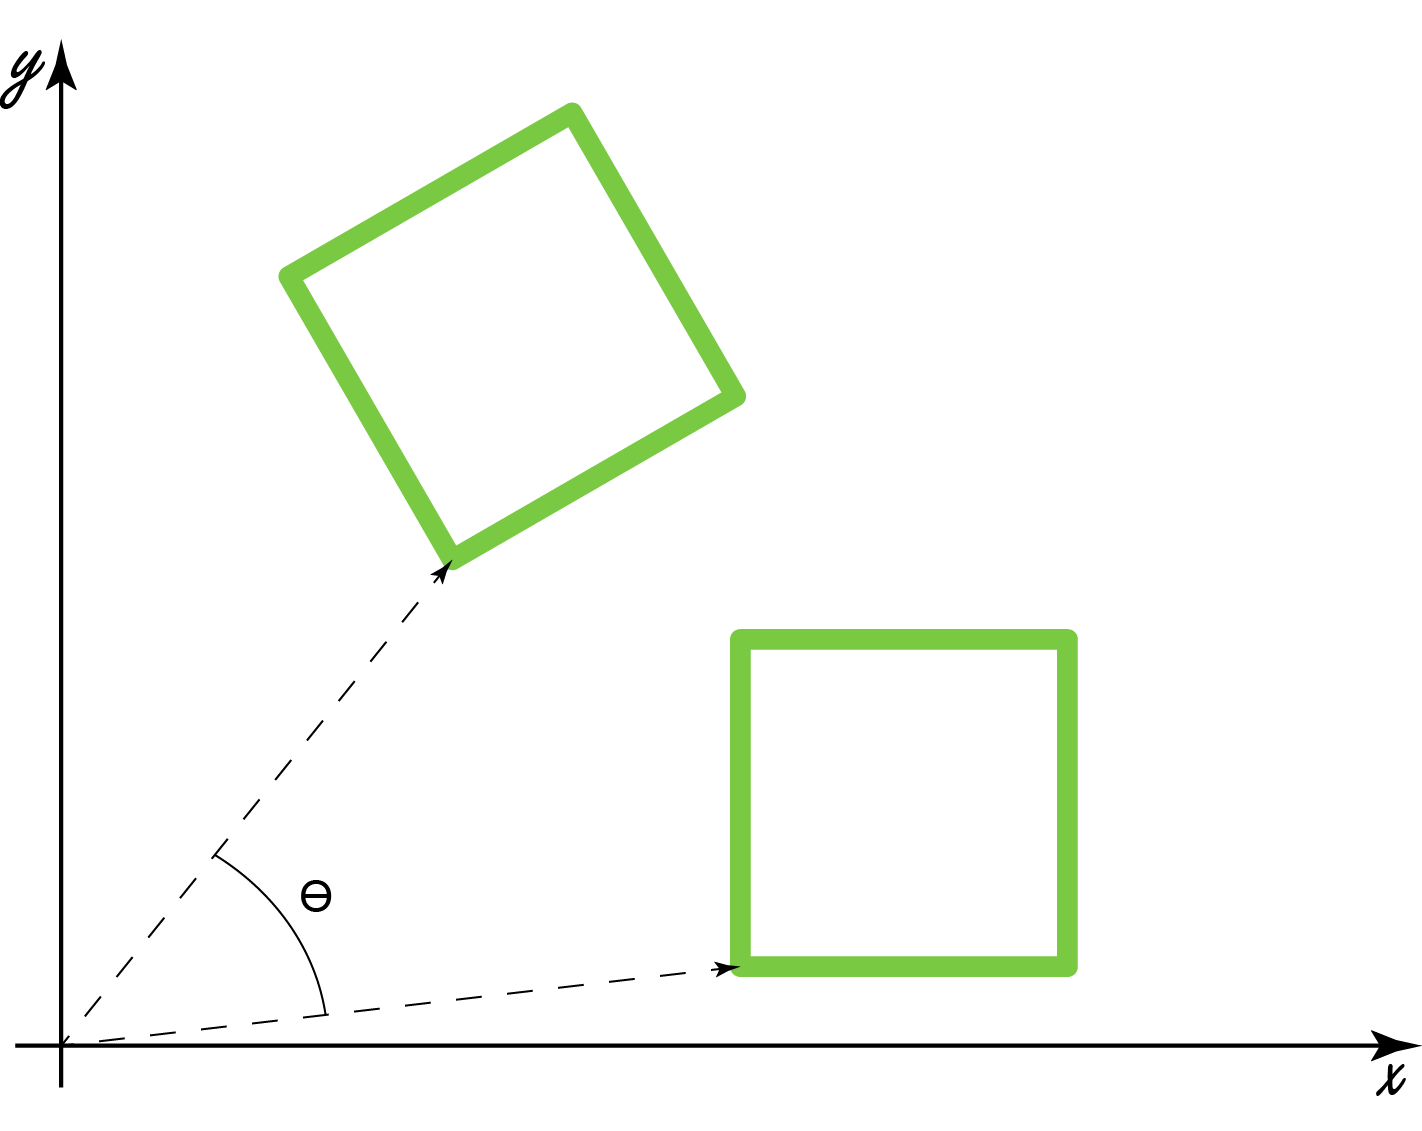
\includegraphics[scale=0.25]{figuras/rotation1}
\caption{Exemplo de rotação em um espaço bidimensional}
\end{center}
\end{figure}

\subsubsection{Cisalhamento}
O cisalhamento resulta em um movimento translacional na direção de um eixo no qual a magnitude aumenta ao longo do outro eixo.

\begin{center}
$\begin{bmatrix}x'\\
y'
\end{bmatrix}=\begin{bmatrix}1 & c\\
1 & 0
\end{bmatrix}\begin{bmatrix}x\\
y
\end{bmatrix}$\end{center}
Onde $c$ é o coeficiente de cisalhamento.\cite{CGPPBook1}

\begin{figure}[H] 
\begin{center}
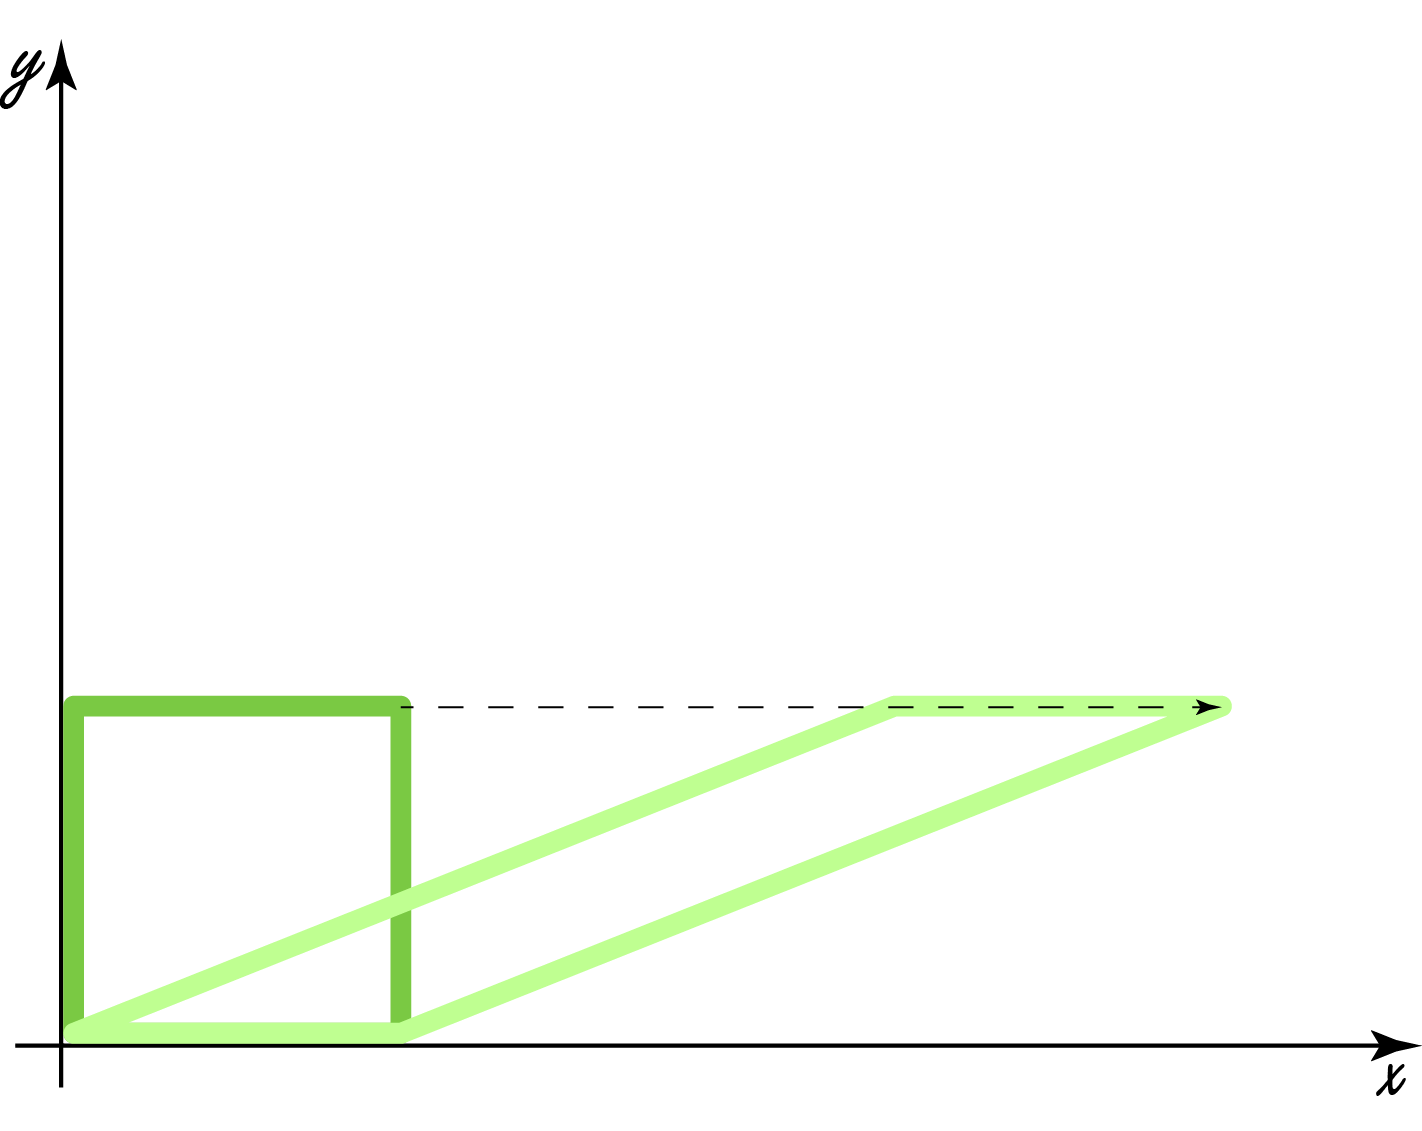
\includegraphics[scale=0.25]{figuras/shear1}
\caption{Exemplo de cisalhamento em um espaço bidimensional}
\end{center}
\end{figure}

\subsubsection{Projeção}
Projeção é o processo no qual se obtém uma figura bidimensional a partir de uma cena tridimensional.\cite{CGPPBook1}


\begin{center}
$\begin{bmatrix}x\\
y\\
z\\
\frac{z}{d}
\end{bmatrix}=\begin{bmatrix}1 & 0 & 0 & 0\\
0 & 1 & 0 & 0\\
0 & 0 & 1 & 0\\
0 & 0 & \frac{1}{d} & 0
\end{bmatrix}\begin{bmatrix}x\\
y\\
z\\
1
\end{bmatrix}$\end{center}

\begin{figure}[H] 
\begin{center}
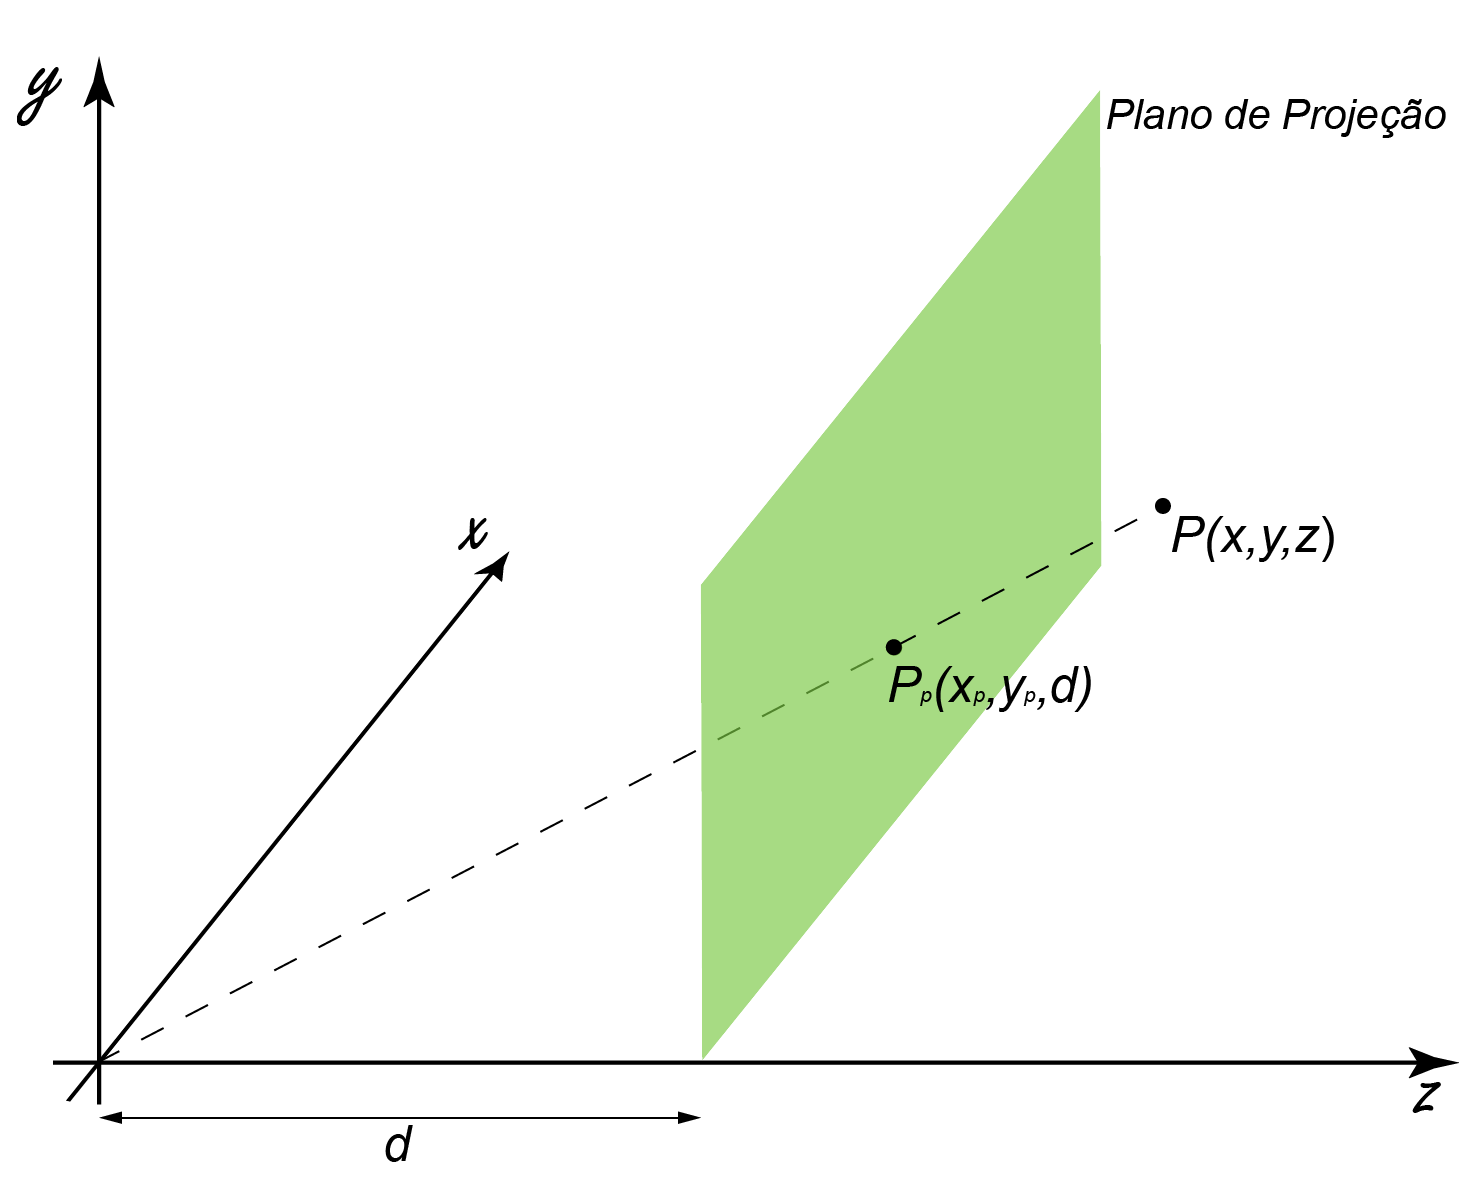
\includegraphics[scale=0.25]{figuras/projection1}
\caption{Exemplo de projeção}
\end{center}
\end{figure}

\subsection{Tipos de transformação}
Existem basicamente quatro tipos de transformações geométricas, mas somente três estão disponíveis no TerraLib:
afim, polinomial de segundo grau e projetiva.
\subsubsection{Linear}

A transformação linear ou também chamada de euclidiana, pode ser definida como:

\begin{center}
$F(x)=Qx$\end{center}
Sendo que $Q=n\times m$.
Ou seja, transformações do tipo lineares são aquelas obtidas através de mutliplicações matriciais.
Assim, através das transformações lineares pode-se realizar operações de rotação, cisalhamento e variação de escala~\cite{CGPPBook1}.

\subsubsection{Afim}
A transformação afim é uma transformação que compreende as operações que a transformação linear consegue executar mais a operação de translação. A transformada em questão pode ser definida como:

\begin{center}
$F(x)=Qx+q$\end{center}
Sendo que $Q=n\times m$ e $q$ tem tamanho $m$ \cite{CGPPBook1}.

\subsubsection{Polinômio de Segundo Grau}
Existe também transformações de segundo grau que são descritas como:
\begin{center}
$F(x)=Wa$\end{center}

\begin{center}
$W=\begin{bmatrix}1 & x_{1} & y_{1} & x_{1}y_{1} & x_{1}^{2} & y_{1}^{2}\\
1 & x_{2} & y_{2} & x_{2}y_{2} & x_{2}^{2} & y_{2}^{2}\\
\vdots & \vdots & \vdots & \vdots & \vdots & \vdots\\
1 & x_{n} & y_{n} & x_{n}y_{n} & x_{n}^{2} & y_{n}^{2}
\end{bmatrix}$\end{center}
Onde $W=n\times m$ e $a$ tem tamanho $m$.\cite{Schowengerdt}

\subsubsection{Projeção}

A projeção é nada mais que uma transformação linear em um espaço projetivo \cite{CGPPBook1}. A forma geral da transformação projetiva é descrita como:

$F(x)=\left( \frac{a_{11}x_{1}+a_{12}x_{2}+...+a_{1n}x_{n}+a_{1n}x_{1(n+1)}}{b_{1}x_{1}+b_{2}x_{2}+...+b_{n}x_{n}+b_{n+1}},\cdots,\right.$

\begin{center}
$\left. \frac{a_{m1}x_{1}+a_{m2}x_{2}+...+a_{mn}x_{n}+a_{mn}x_{m(n+1)}}{b_{1}x_{1}+b_{2}x_{2}+...+b_{n}x_{n}+b_{n+1}} \right)$\end{center}

\section{Avaliação da Precisão do Registro}
Uma operação importante para um sistema de registro é a avaliação da transformação computada. Sejam {g} e {G} as imagens de ajuste e referência respectivamente, e {x, y} e {X, Y} os conjuntos de pontos de controle casados que definem uma transformação de distorção {T}. Pode-se verificar o quão a transformação é correta através do cálculo do erro RMSE.

$$
	RMSE = \sqrt{\frac{1}{n}\sum\limits_{i=1}^{n}(x_i - T(X_i))^2 + (y_i - T(Y_i))^2}
$$

onde:

$(x_i, y_i), (X_i, Y_i)$, $i = 1..n$ é o conjunto de pares de pontos de contole obtidos no processo de casamento.
$T$ é a função de distorção entre as imagens obtida através do casamento de pontos de controle.\cite{Fedorov1}

\section{ Sistema Automático Para Registro e Mosaico }
 
O sistema implementado está separado em duas partes baseados em algoritmos do Terralib: a) A primeira parte se refere ao bloco \texttt{MMIOMatching} e \texttt{OFMatching}, onde duas imagens são utilizados como parâmetros do bloco e como resultado são apresentados o registro e extração dos pontos de controles. Esses pontos de controle são representados através de dois vetores para calculo da função de transformação, onde são localizados e acrescentados na nova imagem resultante. b) A Segunda parte se refere ao bloco Mosaic, que recebe como parâmetros de entrada a saída do primeiro bloco, ou seja, os vetores  que representam os pontos de controle. Além disso, são parâmetros de entrada as imagens que serão mosaicadas e o nome da nova imagem que apresentará o resultado do mosaico. Veja a Figura~\ref{fig:estrutura_logica} que apresenta a estrutura lógica de funcionamento do sistema.

\begin{figure}[h!t]
\begin{center}
\includegraphics[scale=0.50]{figuras/estrutura_logica}
\caption{Estrutura Lógica do Sistema}
\label{fig:estrutura_logica}
\end{center} 
\end{figure}

Foram realizados vários testes empíricos, e para alcançarmos resultados satisfatórios desenvolvemos um sistema hibrido utilizando os dois métodos de registro. O método \texttt{MMIOMatching} apresentou resultados melhores para os testes realizados, todavia é mais lento que o método \texttt{OFMatching}. Este último método, foi o mais rápido para realização do registro, e em algumas cenas, embora apresentasse o valor de erro RMSE baixo, encontrava poucos pontos de controle, e por consequência o mosaico utilizando esses pontos apresentavam grandes distorções. Através dos testes realizados chegamos a seguinte configuração:

\subsection{Configuração do Sistema}
\begin{enumerate}
\item MMIOMatching
	\begin{enumerate}
	 \item Tipo de transformação geométrica: Afim.
	 \item Estratégia de Remoção de pontos divergentes: Remoção aleatória.
	 \item Valores máximos para os erros de mapeamento (direto e inverso): 5.
	 \item Relação de resolução entre pixels: 1 para 1.
	 \item Número máximo de pontos de controles a ser localizados: 4000 pontos.
	 \item Tamanho da janela de correlação: 45x45 pixels.
	 \item Tamanho da janela do Operador Moravec :11x11 pixels.
	\end{enumerate}
 \item OFMatching
	 \begin{enumerate}
	  \item Tipo de transformação geométrica: Afim.
	  \item Estratégia de Remoção de pontos divergentes: Remoção aleatória.
	  \item Valores máximos para os erros de mapeamento (direto e inverso): 5.
	  \item Relação de resolução entre pixels: 1 para 1.
	  \item Número máximo de pontos de controles a ser localizados: 529.
	  \item Tamanho da janela de correlação: 45.
	  \item Sensibilidade da correlação: 0.5.
	  \item Máxima sensibilidade de detecção: 0.02.
	 \end{enumerate}
 \item Mosaic
	 \begin{enumerate}
	  \item Método de mistura (Blender): Sem blender.
	  \item Método de interpolação: Vizinhos mais próximos.
	  \item Opçao de autoequalização (com ou sem): com equalização.
	 \end{enumerate}
\end{enumerate}

O sistema registra e mosaica as imagens de maneira automática, e para isso é apenas informado o caminho da pasta que contém as imagens a serem registradas e mosaicadas. Cada mosaico gerado é salvo dentro dessa mesma pasta.

A heurística para a escolha do algoritmo de registro começa primeiramente executando o registro utilizando o método \texttt{OFMatching} por ser mais rápido. Ao final do registro é analisado o valor do erro RMSE e a quantidade de pontos encontrados. Se a quantidade de pontos e o valor do erro RMSE satisfazer um determinado limiar, então efetua-se o mosaico de duas imagens utilizando os pontos de controle e a transformação geométrica calculada. O processo é reinciado até que acabe a lista de imagens selecionadas para a realização de registro e mosaico.

Todavia, se a quantidade de pontos de controle e o erro RMSE não atenderem ao limiar definido, então é executado o algoritmo \texttt{MMIOMatching} para encontrar os novos pontos de controle e em seguida o mosaico das duas imagens através dos novos valores calculados, e o processo é reiniciado.

\section{Resultados}

As imagens analisadas foram coletadas por uma câmera digital a bordo de um VANT, e apresentam muito ruído devido ao formato de compressão ser JPEG. A Figura~\ref{fig:mosaico} foi conseguida através do registro e mosaico de 14 imagens JPEG com tamanho de 4000 x 3000 pixels, consumindo quase 4 horas para o processamento. Essas imagens foram selecionadas para compor os testes realizados neste trabalho por apresentarem diversas rotações devido serem captadas durante o momento em que o VANT efetua curvas para seguir o plano de voo.

\begin{figure*}[!b]
\begin{center}
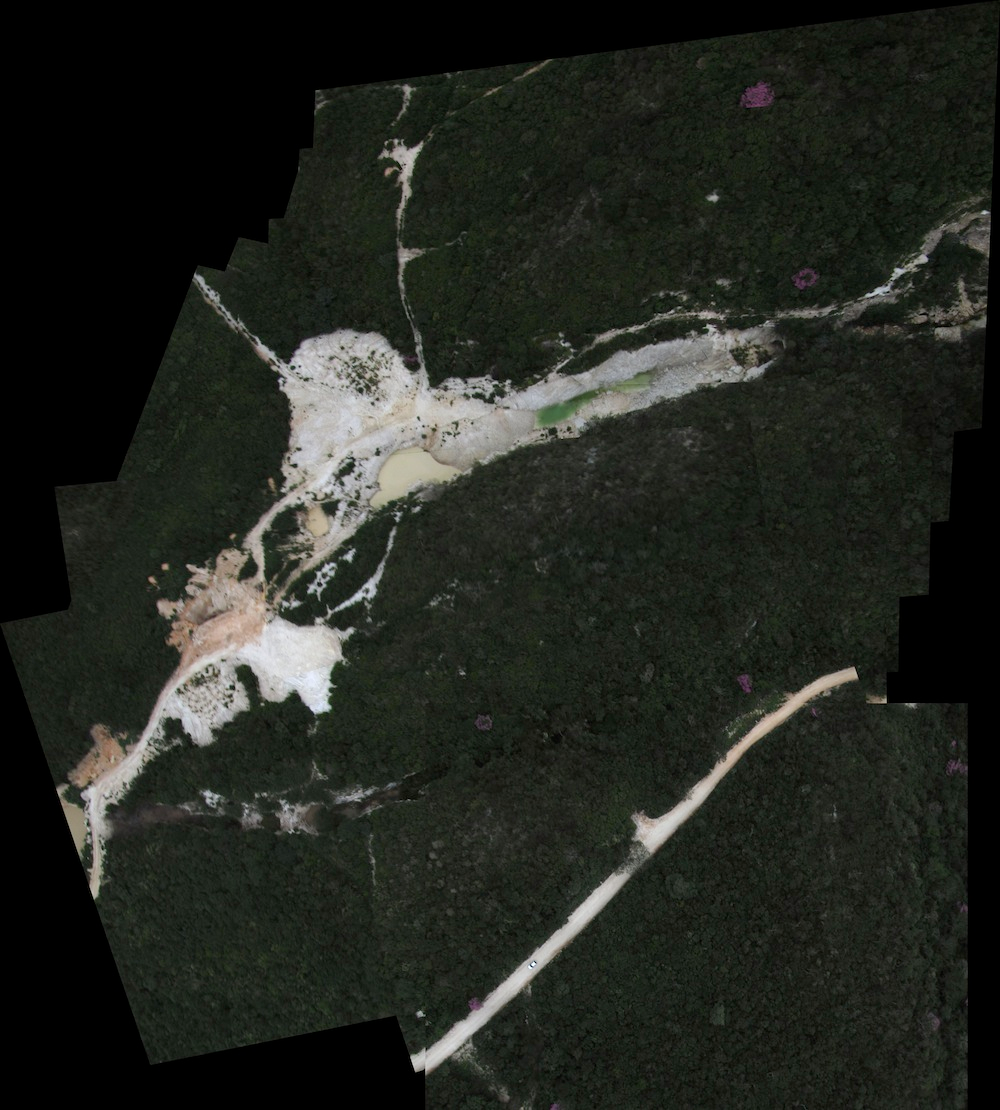
\includegraphics[scale=0.30]{figuras/mosaico}
\caption{Mosaico de 12 imagens}
\label{fig:mosaico}
\end{center}
\end{figure*}

A Tabela~\ref{tab:resultados} apresenta a quantidade de pontos de controle encontrados pelo algoritmo, os valores de erro RMSE para mapeamento direto e inverso, tempo de processamento, imagens que comporam o processamento e se o resultado foi ou não aceito. Os resultados foram conseguidos executando a implementação em um laptop com processador Intel Core i5 de 2,4 GHz com dois núcleos de processamento e 4 GB de memória ram 1333 MHz DDR3.

Analisando os resultados, percebemos que o algoritmo \texttt{OFMatching} embora muito rápido, obteve poucos resultados aceitos, porém isso não significa que o algoritmo não é bom para realizar registro de imagens aéreas. Esse algoritmo não obteve muito sucesso devido as imagens escolhidas serem as mais difíceis de registrar, todavia em outros testes executados em imagens que não apresentavam muito ruído e rotações, esse algoritmo foi muito bem sucedido. Embora mais lento, o algoritmo \texttt{MMIOMatching} foi o que obteve os melhores resultados.

\begin{table*}[!hb]
\small
\caption{Registro e Mosaico de Imagens Aéreas}
\begin{center}
\begin{tabular}{ccccccc}
\hline\hline
Algoritmo   & Qtd Pontos    &RMSE direto   &RMSE inverso    &Tempo de processamento   &Imagens   & Resultado aceito\\
\hline\hline
OFMatching	&6	&2.32	&2.31	&39 segundos	&img1 e img2 &sim\\
\hline
OFMatching	&3	&7.68e-13	&6.99e-12	&49 segundos	&mos1 e img3 &\\
MMIOMatching	&11	&2.21	&2.77	&492 segundos	&mos1 e img3 &sim\\
\hline
OFMatching	&3	&3.69e-12	&1.37e-11	&74 segundos	&mos2 e img4 &\\
MMIOMatching	&58	&2.62	&3.14	&755 segundos	&mos2 e img4 &sim\\
\hline
OFMatching	&4	&0.82	&0.89	&85 segundos	&mos3 e img5 &\\
MMIOMatching	&66	&2.73	&3.12	&861 segundos	&mos3 e img5 &sim\\
\hline
OFMatching	&4	&1.21	&1.20	&84 segundos	&mos4 e img6 &\\
MMIOMatching	&63	&2.91	&3.17	&901 segundos	&mos4 e img6 &sim\\
\hline
OFMatching	&3	&8.30e-13	&8.52e-10	&79 segundos	&mos5 e img7 &\\
MMIOMatching	&97	&2.49	&2.81	&1032 segundos	&mos5 e img7 &sim\\
\hline
OFMatching	&4	&2.08	&2.21	&101 segundos	&mos6 e img8 &\\
MMIOMatching	&93	&2.53	&2.89	&1069 segundos	&mos6 e img8 &sim\\
\hline
OFMatching	&4	&0.63	&0.80	&107 segundos	&mos7 e img9 &\\
MMIOMatching	&61	&2.58	&2.88	&1216 segundos	&mos7 e img9 &sim\\
\hline
OFMatching	&4	&1.39	&2.36	&120 segundos	&mos8 e img10 &\\
MMIOMatching	&48	&2.75	&3.12	&1295 segundos	&mos8 e img10 &sim\\
\hline
OFMatching	&5	&2.26	&2.20	&129 segundos	&mos9 e img11 &sim\\
\hline
OFMatching	&3	&3.82e-12	&4.21e-10	&138 segundos	&mos10 e img12 &\\
MMIOMatching	&61	&3.01	&3.12	&1401 segundos	&mos10 e img12 &sim\\
\hline
OFMatching	&3	&2.69e-12	&1.55e-11	&131 segundos	&mos11 e img13&\\
MMIOMatching	&64	&2.77	&2.99	&1391 segundos	&mos11 e img13 &sim\\
\hline
OFMatching	&4	&0.70	&1.09	&135 segundos	&mos12 e img14&\\
MMIOMatching	&38	&2.78	&2.96	&1456 segundos	&mos12 e img14 &sim\\
\hline\hline
\end{tabular}
\label{tab:resultados}
\end{center}
\end{table*}

\section{Conclusão}
No trabalho foram apresentados os resultados de testes referentes ao mosaico de seqüências de imagens aéreas, onde procuramos aumentar a qualidade e a velocidade dos processos de mosaico e registros. Os testes se basearam em algoritmos implementados na biblioteca TerraLib e apresentaram resultados satisfatórios, porém com tempo de processamento muito alto.

\bibliographystyle{IEEEbib}
\bibliography{biblio}

\clearpage

\begin{figure}[!h]
\begin{center}
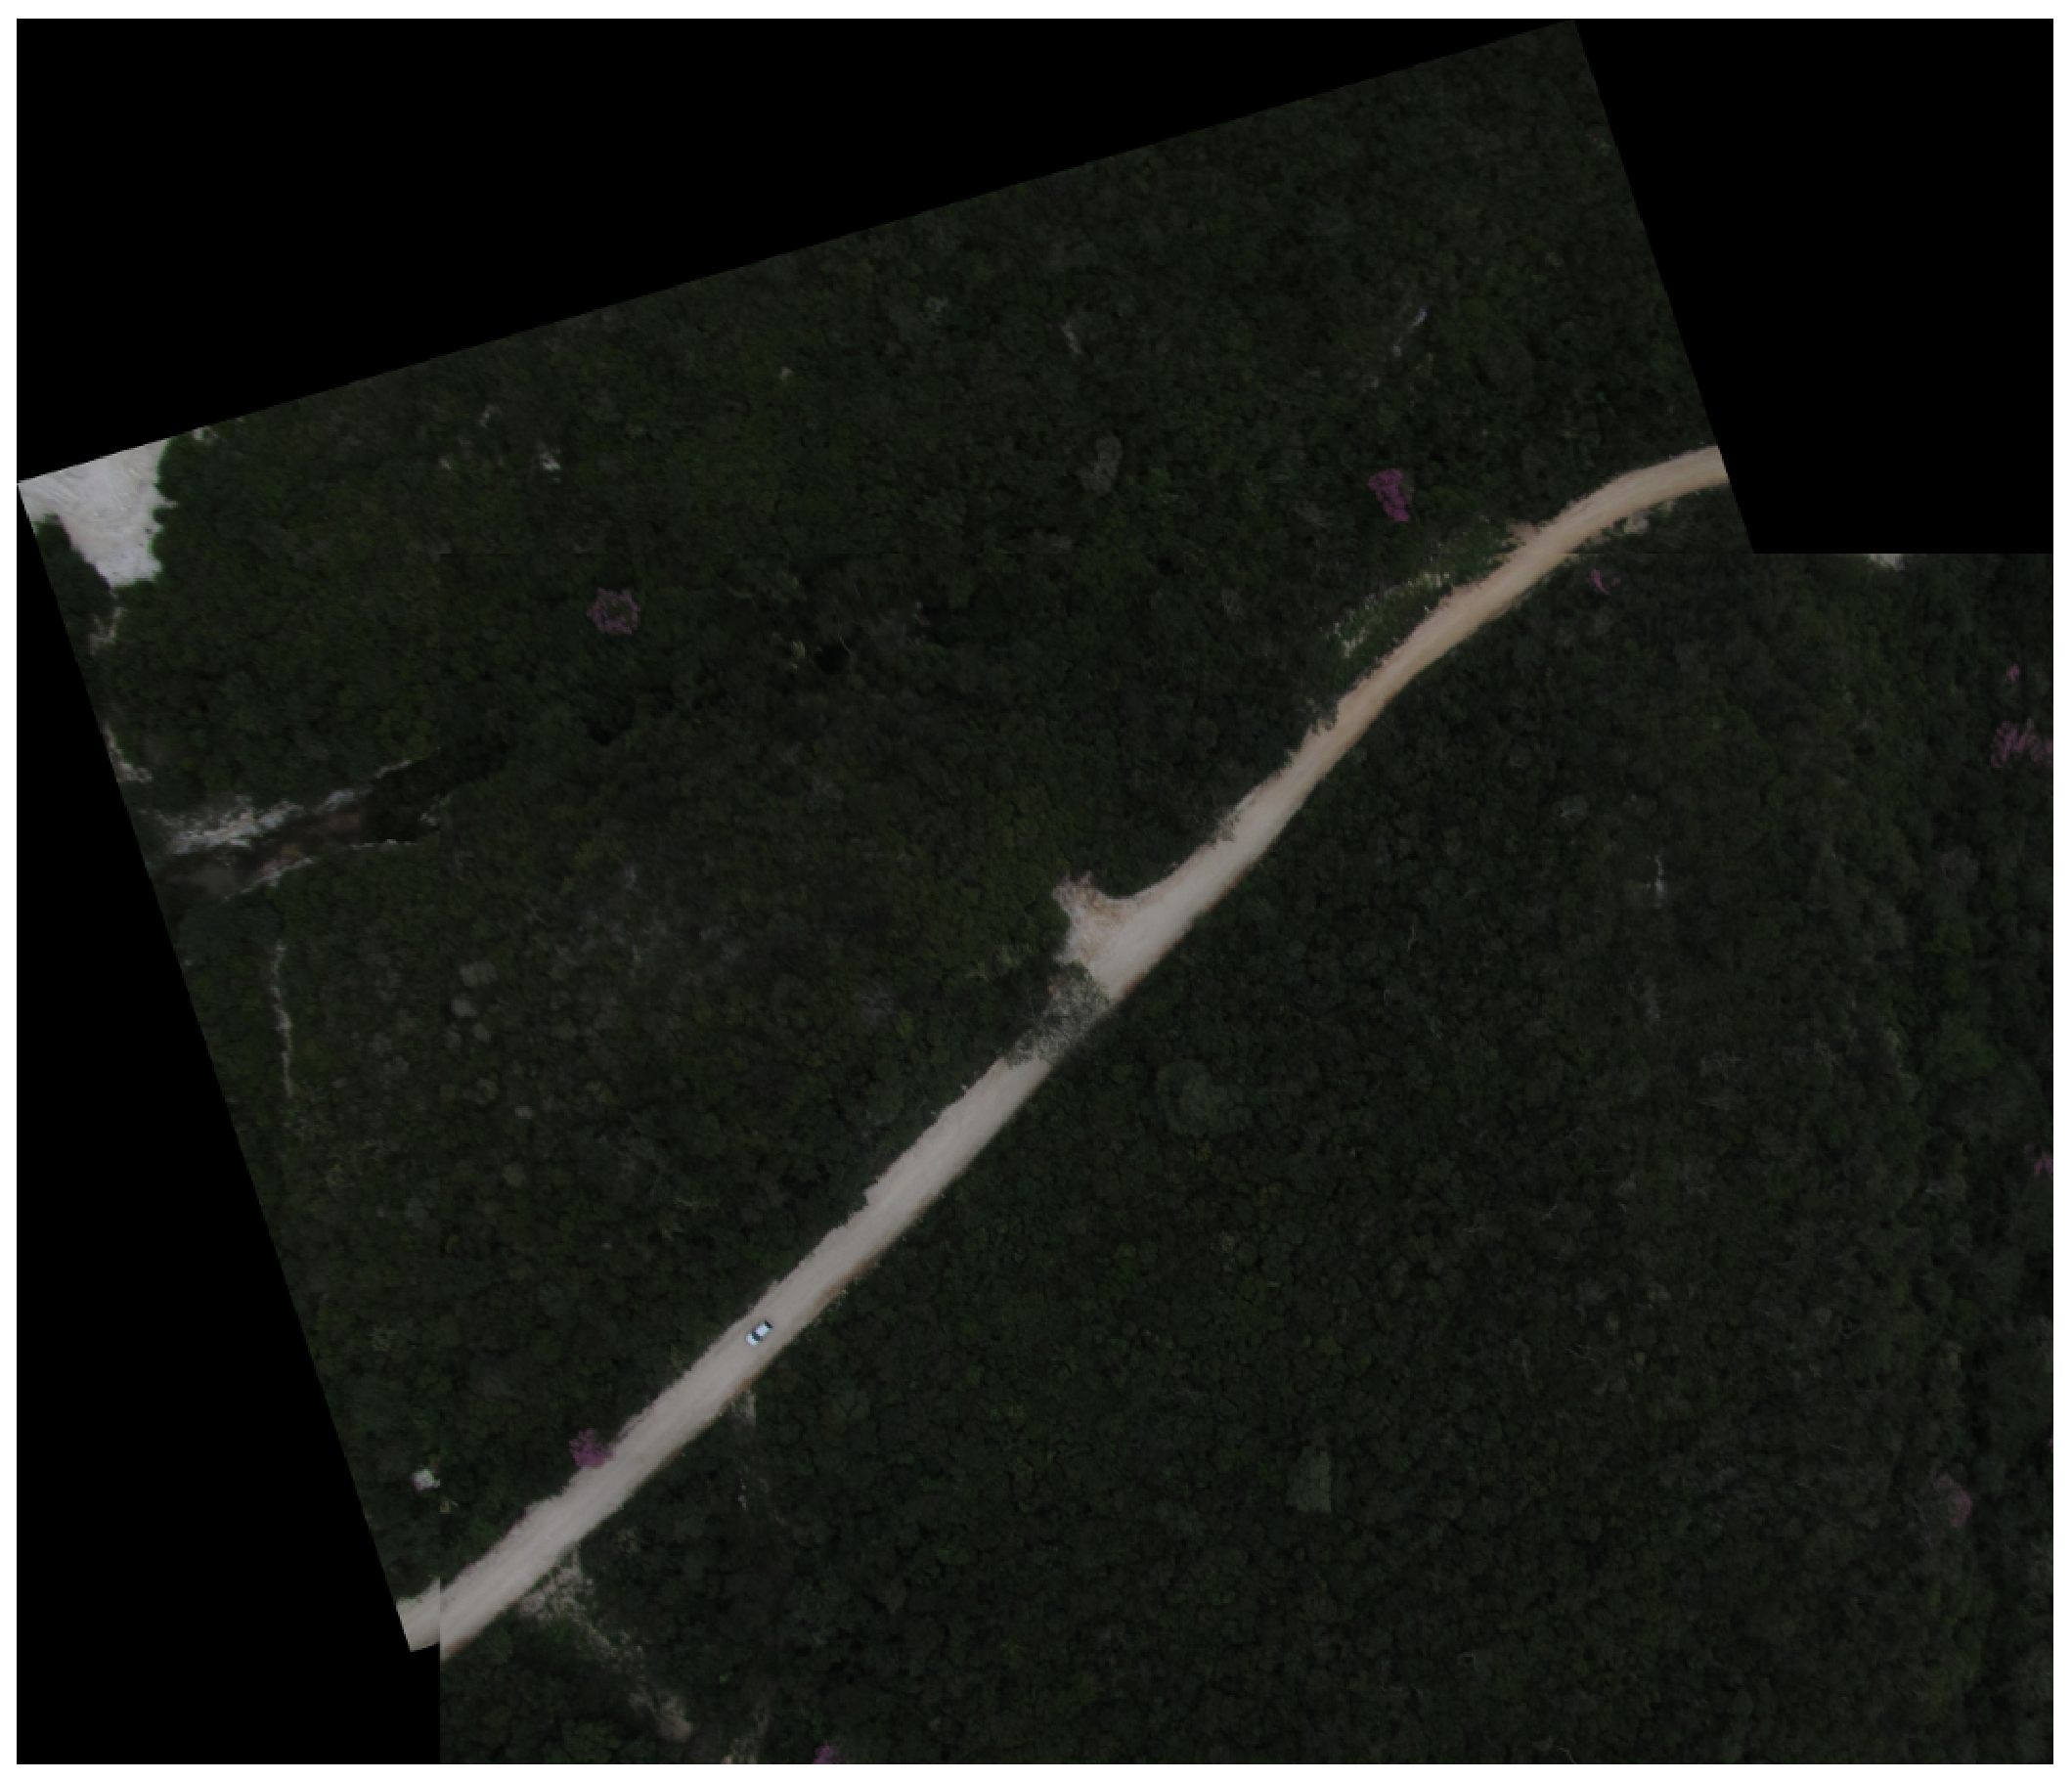
\includegraphics[scale=0.25]{figuras/Mosaic0}
\caption{Mosaico parcial - Img1 e Img2}
\label{fig:mosaico}
\end{center}
\end{figure}

\begin{figure}[!h]
\begin{center}
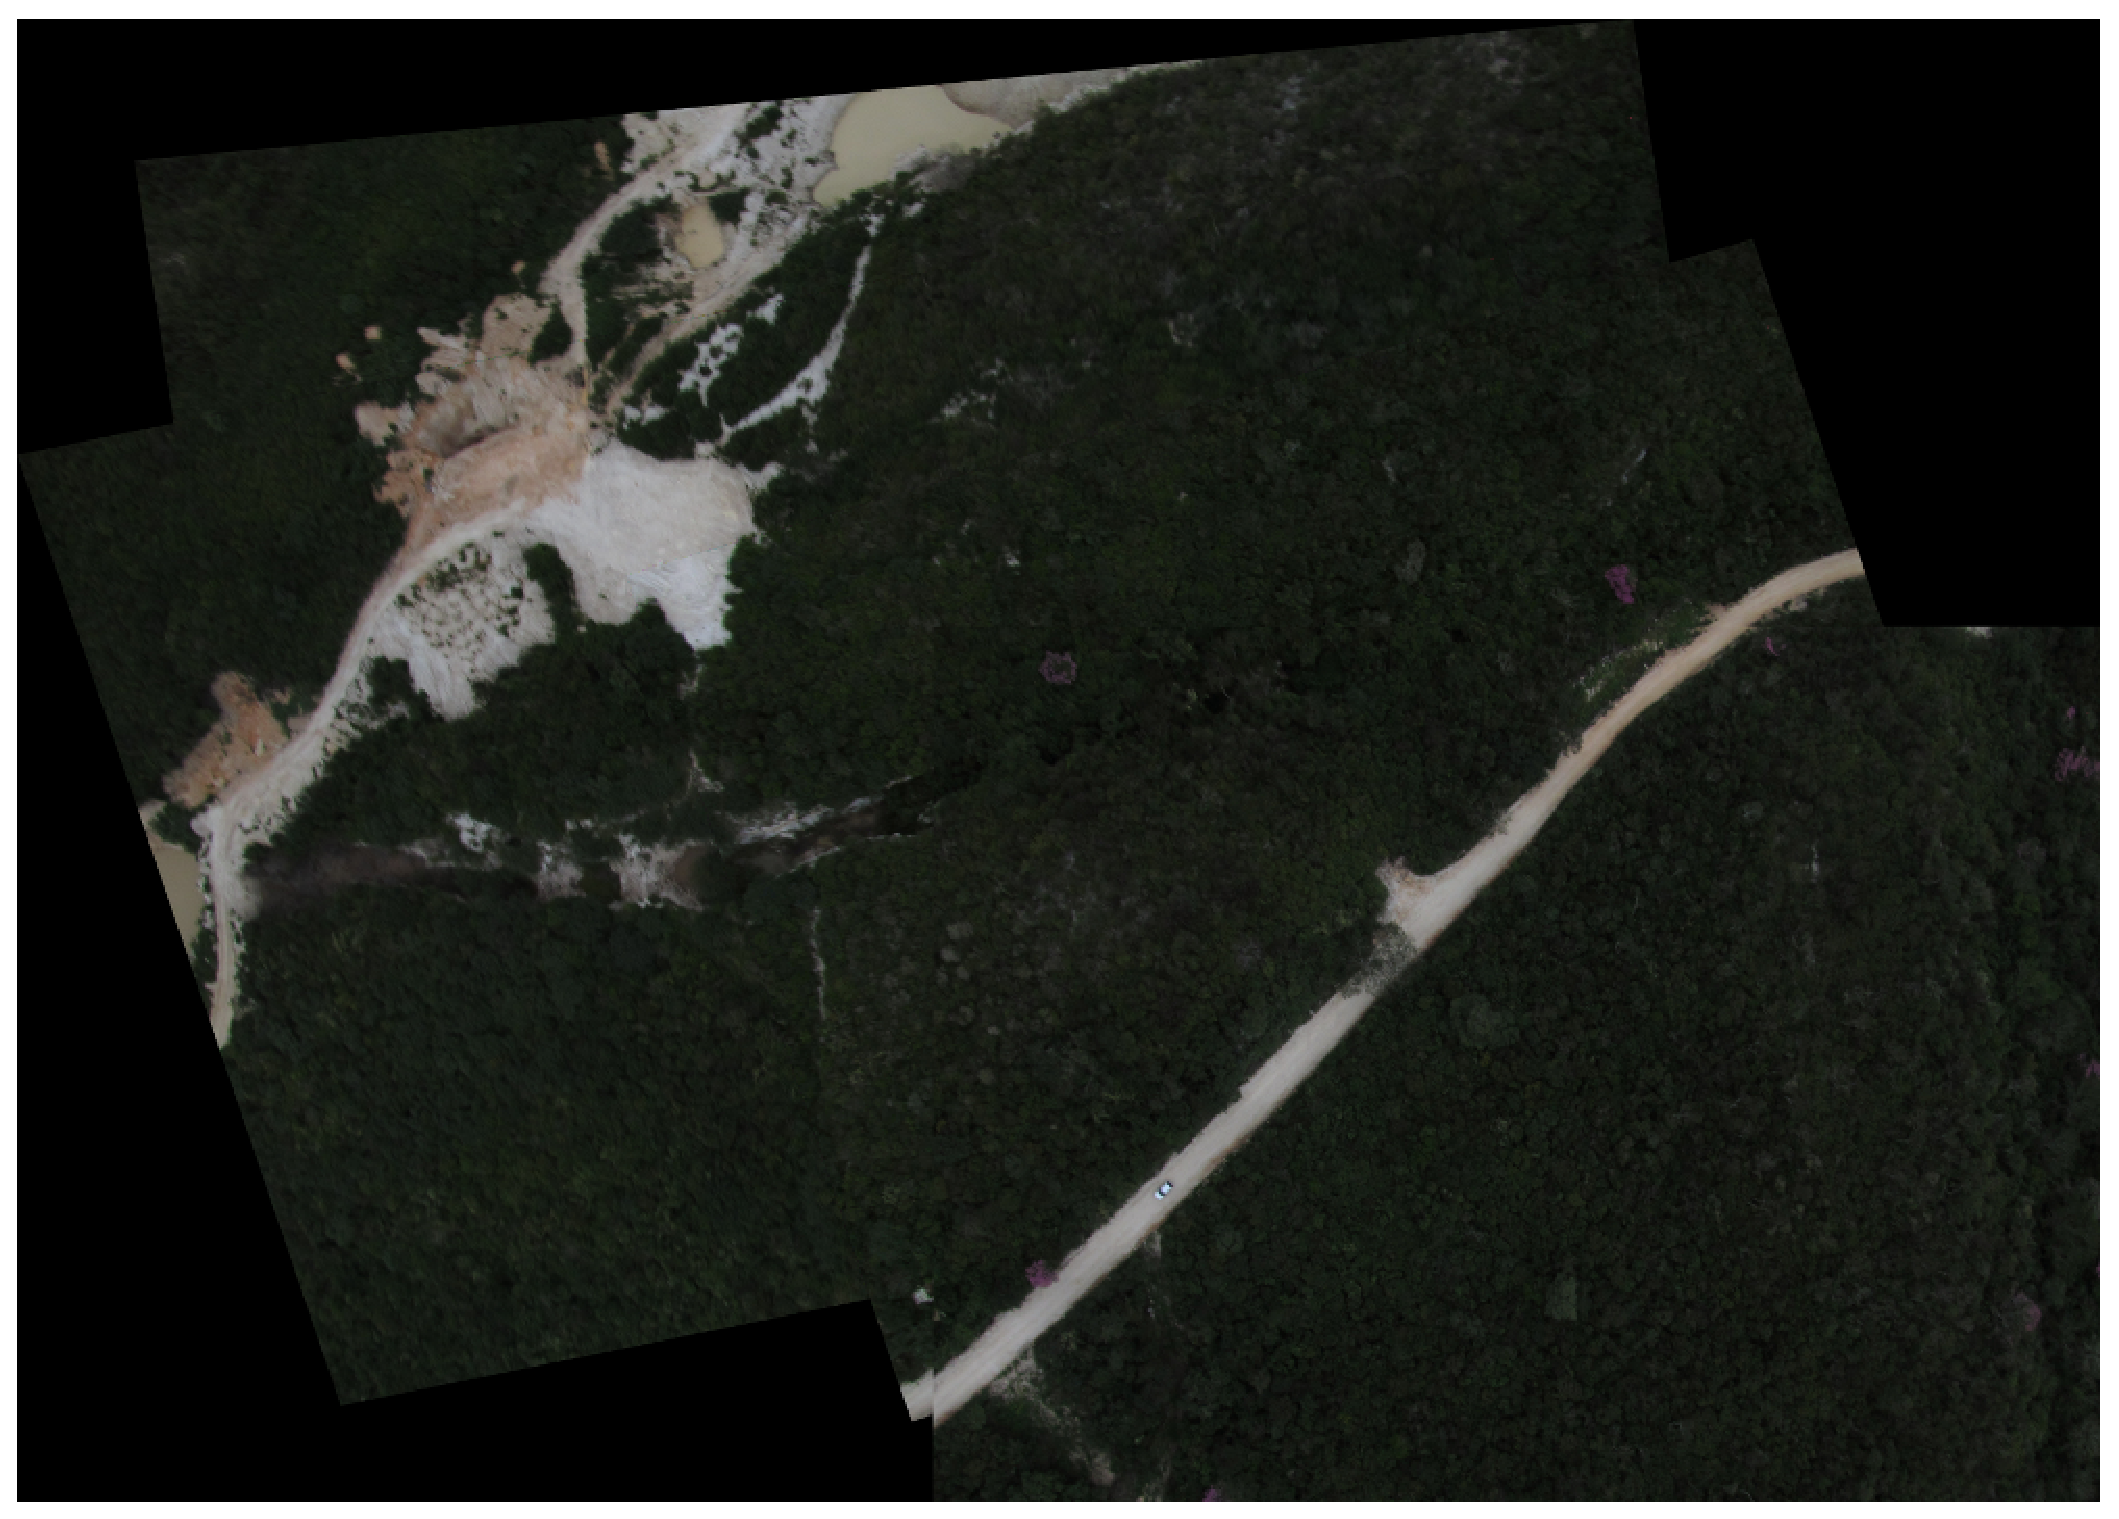
\includegraphics[scale=0.25]{figuras/Mosaic2}
\caption{Mosaico parcial - Mos1 e Img3 }
\label{fig:mosaico}
\end{center}
\end{figure}

\begin{figure}[!h]
\begin{center}
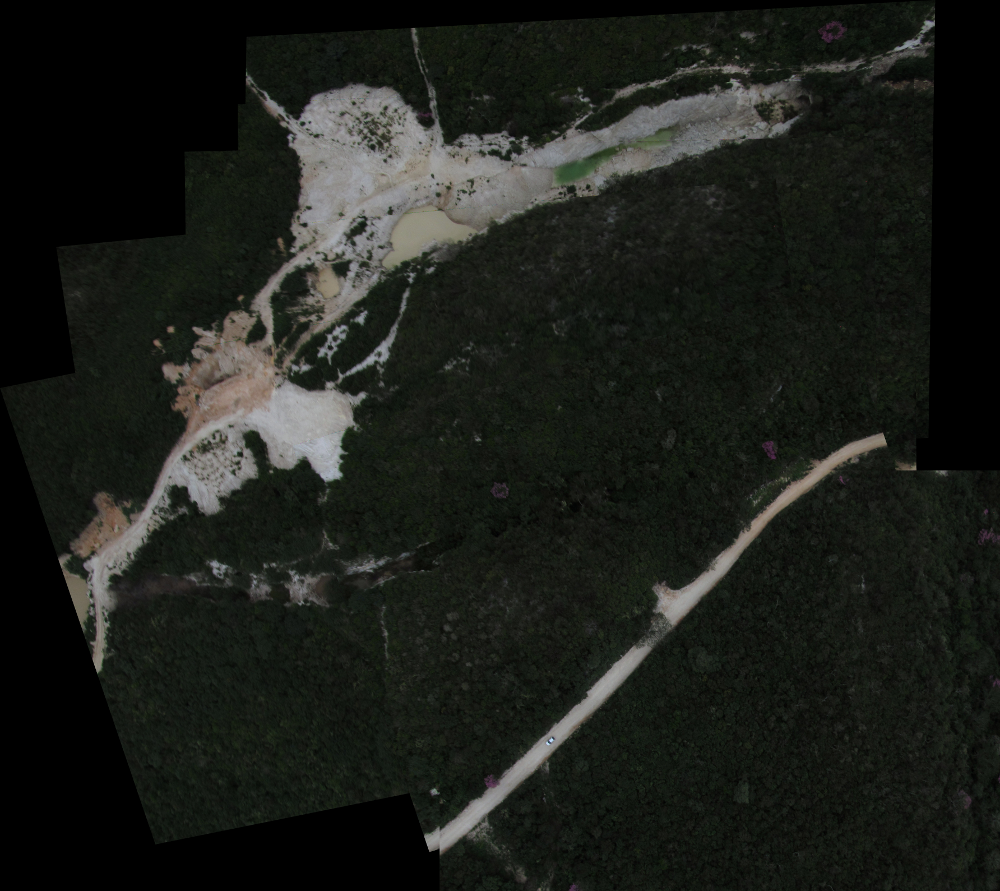
\includegraphics[scale=0.25]{figuras/Mosaic5}
\caption{Mosaico parcial - Mos4 e Img6}
\label{fig:mosaico}
\end{center}
\end{figure}



\begin{figure}[!h]
\begin{center}
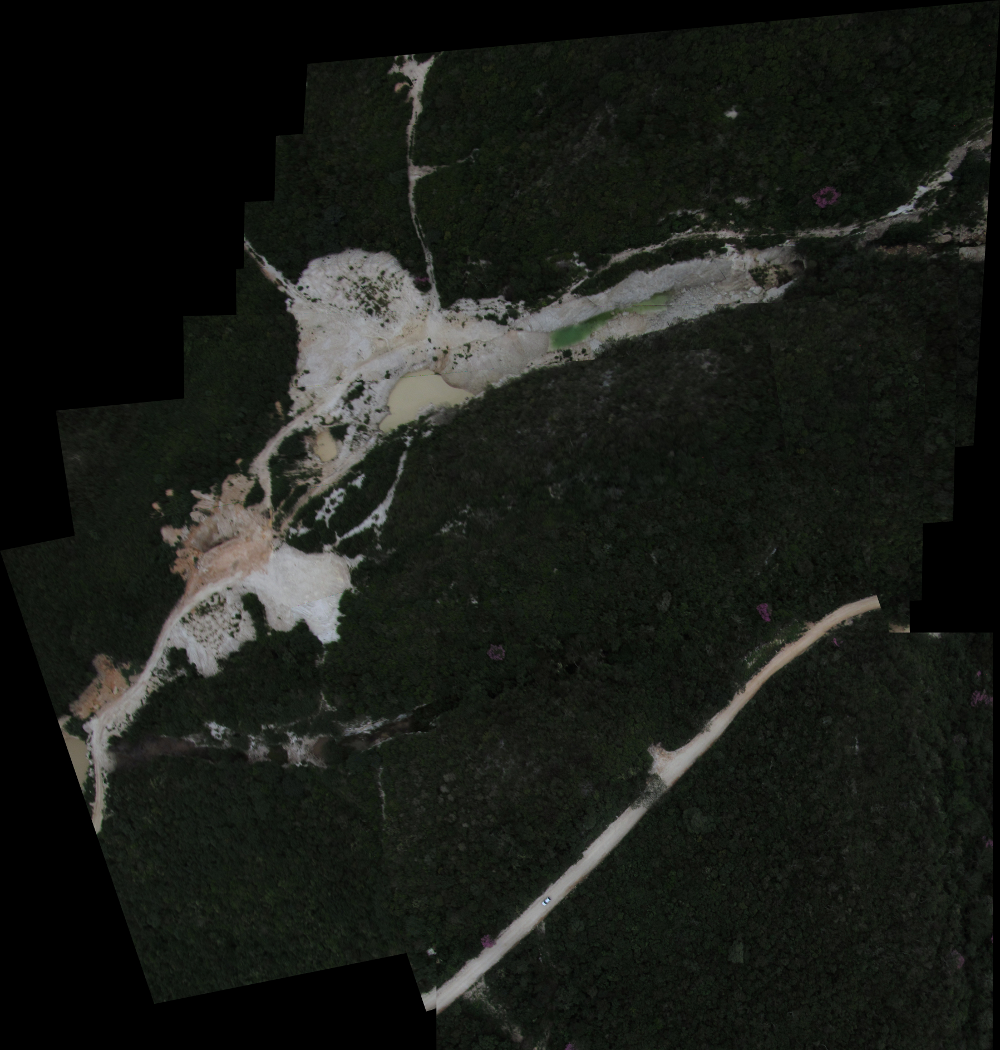
\includegraphics[scale=0.25]{figuras/Mosaic7}
\caption{Mosaico parcial - Mos6 e Img8}
\label{fig:mosaico}
\end{center}
\end{figure}

\end{document}

